%======================================================================
\chapter{Python: Qt-Material}\label{appendix:qt-material}

\begin{description}
   \item[Description:]      Material inspired stylesheet for PySide2, PySide6, PyQt5 and PyQt6.
   \item[License:]          BSD-2-clause
   \item[Latest version:]   \quot{2.12}
   \item[Python:]           \quot{3.8, 3.9, 3.10}
   \item[PyPi:]             \url{https://pypi.org/project/qt-material/}
   \item[Repository:]       \url{https://github.com/UN-GCPDS/qt-material}
   \item[Documentation:]    \url{https://qt-material.readthedocs.io/en/latest/}
\end{description}
\hrulefill

This is another stylesheet for PySide6, PySide2, PyQt5 and PyQt6, which looks like Material Design (close enough).

\begin{figure}
\begin{centering}
% \includesvg[width=0.8\textwidth]{Cap4/Figures/transformer.svg}
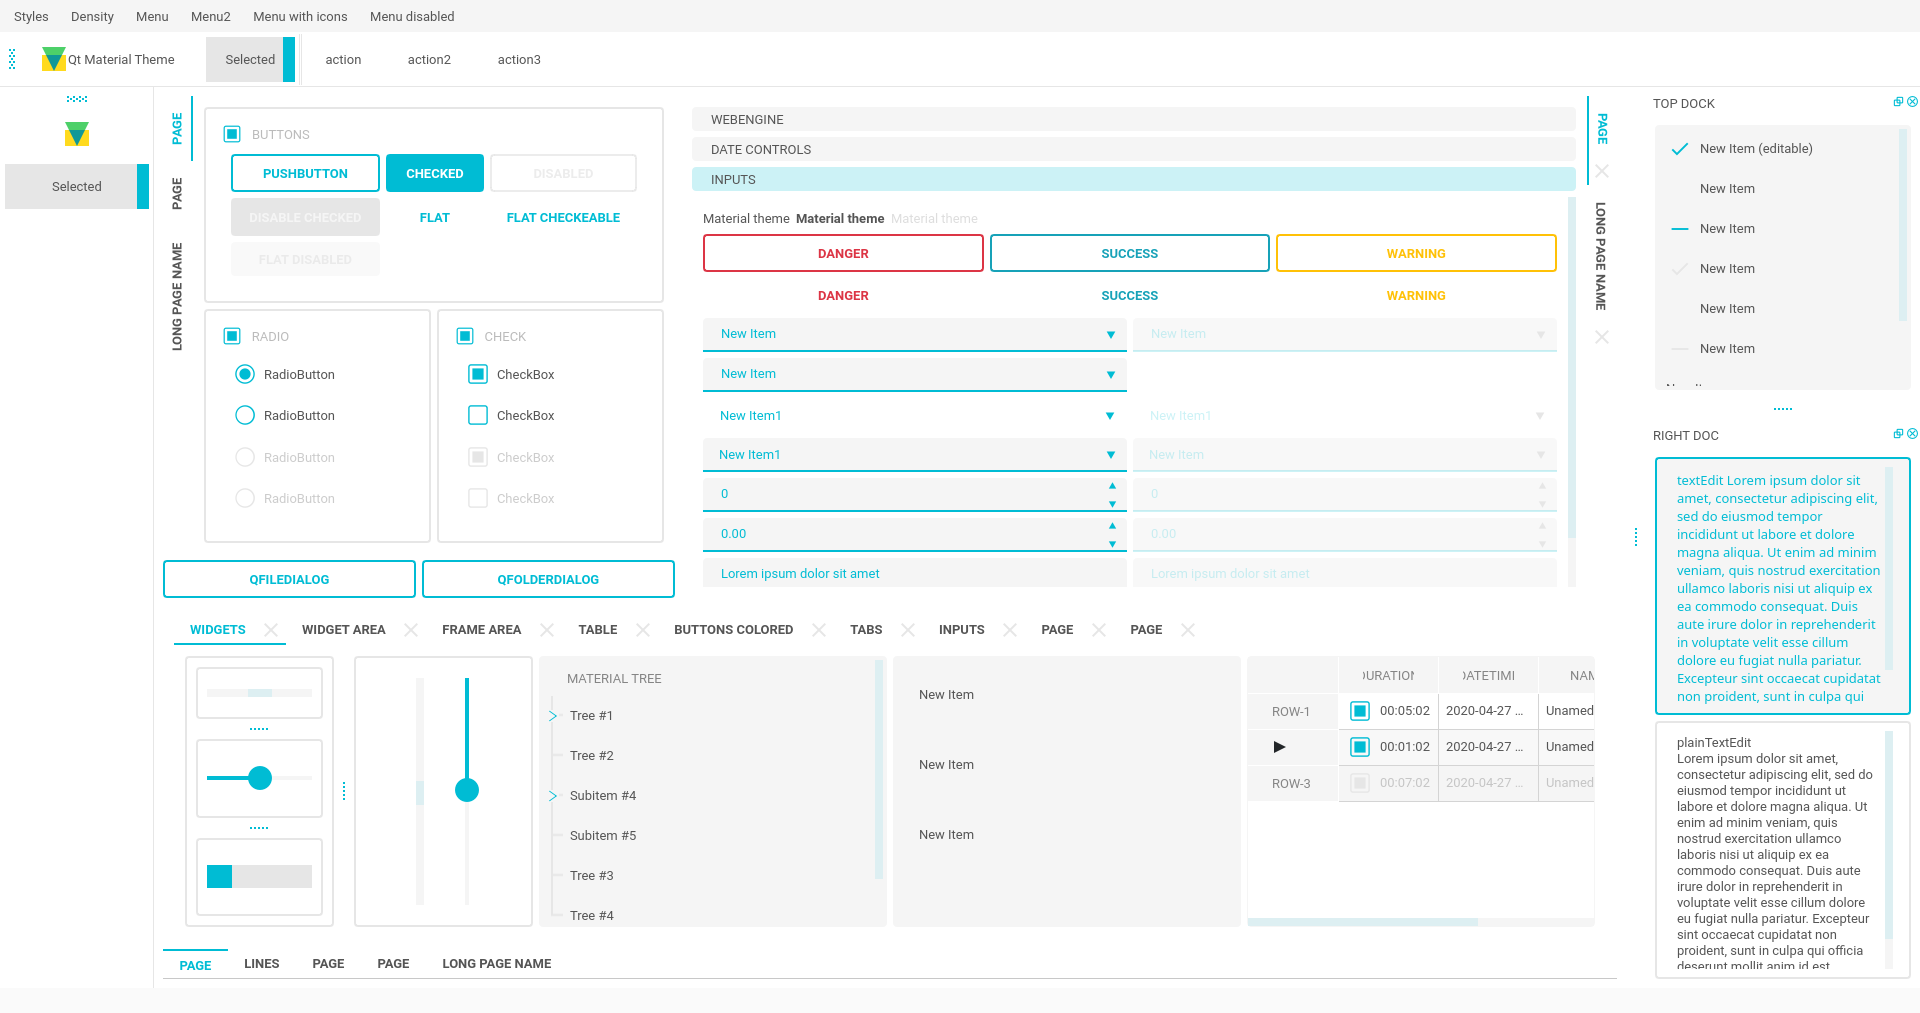
\includegraphics[width=1\textwidth]{Appendix/python_modules/Figures/qt-light_cyan_500.png}
\par\end{centering}
\caption[\textit{light\_cyan\_500.xml} theme for Qt-Material]{\textit{light\_cyan\_500.xml} theme for Qt-Material.}
\label{fig:qt-light_cyan_500}
\end{figure}

%======================================================================
\section{Install}
\begin{python}
pip install -U qt-material
\end{python}

%======================================================================
\section{Usage}
\begin{python}
import sys
from PySide6 import QtWidgets
# from PySide2 import QtWidgets
# from PyQt5 import QtWidgets
from qt_material import apply_stylesheet

# create the application and the main window
app = QtWidgets.QApplication(sys.argv)
window = QtWidgets.QMainWindow()

# setup stylesheet
apply_stylesheet(app, theme='dark_teal.xml')

# run
window.show()
app.exec_()
\end{python}
\
%======================================================================
\section{Themes}
\begin{python}
from qt_material import list_themes

list_themes()
\end{python}
\begin{python}
['dark_amber.xml',
 'dark_blue.xml',
 'dark_cyan.xml',
 'dark_lightgreen.xml',
 'dark_pink.xml',
 'dark_purple.xml',
 'dark_red.xml',
 'dark_teal.xml',
 'dark_yellow.xml',
 'light_amber.xml',
 'light_blue.xml',
 'light_cyan.xml',
 'light_cyan_500.xml',
 'light_lightgreen.xml',
 'light_pink.xml',
 'light_purple.xml',
 'light_red.xml',
 'light_teal.xml',
 'light_yellow.xml']
\end{python}

%======================================================================
\section{Custom colors}
\footcite{Color Tool}{https://material.io/resources/color/#!/?view.left=0&view.right=0} is the best way to generate new themes, just choose colors and export as \quot{Android XML}, the theme file must look like:
\begin{python}
<!--?xml version="1.0" encoding="UTF-8"?-->
<resources>
<color name="primaryColor">#00e5ff</color>
<color name="primaryLightColor">#6effff</color>
<color name="secondaryColor">#f5f5f5</color>
<color name="secondaryLightColor">#ffffff</color>
<color name="secondaryDarkColor">#e6e6e6</color>
<color name="primaryTextColor">#000000</color>
<color name="secondaryTextColor">#000000</color>
</resources>
\end{python}

Save it as \quot{my\_theme.xml} or similar and apply the style sheet from Python.

\begin{python}
apply_stylesheet(app, theme='dark_teal.xml')
\end{python}


%======================================================================
\section{Light themes}
Light themes will need to add \quot{invert\_secondary} argument as \quot{True}.
\begin{python}
apply_stylesheet(app, theme='light_red.xml', invert_secondary=True)
\end{python}


%======================================================================
\section{Environ variables}
There is a environ variables related to the current theme used, these variables are for consult purpose only.

% Preview source code for paragraph 18

\begin{table}[H]
\begin{centering}
\begin{tabular}{>{\raggedright}m{5cm}>{\raggedright}m{5cm}>{\raggedright}m{2cm}}
\toprule 
\addlinespace[1em]
\textbf{Environ variable} & \textbf{Description} & \textbf{Example}\tabularnewline\addlinespace[1em]
\midrule
\quottable{QTMATERIAL\_PRIMARYCOLOR}  & Primary color  & \quottable{\#2979ff}\tabularnewline
\addlinespace[0.5cm]
\quottable{QTMATERIAL\_PRIMARYLIGHTCOLOR} & A bright version of the primary color & \quottable{\#75a7ff}\tabularnewline
\addlinespace[0.5cm]
\quottable{QTMATERIAL\_SECONDARYCOLOR} & Secondary color & \quottable{\#f5f5f5}\tabularnewline
\addlinespace[0.5cm]
\quottable{QTMATERIAL\_SECONDARYLIGHTCOLOR}  & A bright version of the secondary color  & \quottable{\#ffffff} \tabularnewline
\addlinespace[0.5cm]
\quottable{QTMATERIAL\_SECONDARYDARKCOLOR}  & A dark version of the primary color  & \quottable{\#e6e6e6} \tabularnewline
\addlinespace[0.5cm]
\quottable{QTMATERIAL\_PRIMARYTEXTCOLOR}  & Color for text over primary background  & \quottable{\#000000} \tabularnewline
\addlinespace[0.5cm]
\quottable{QTMATERIAL\_SECONDARYTEXTCOLOR} & Color for text over secondary background  & \quottable{\#000000} \tabularnewline
\addlinespace[0.5cm]
\quottable{QTMATERIAL\_THEME} & Name of theme used  & \quottable{"light\_blue.xml"}\tabularnewline
\bottomrule
\addlinespace[0.5cm]
\end{tabular}
\par\end{centering}
\caption{Environ variables defined by Qt-Material.\label{table:environ_vars}}
\end{table}



%======================================================================
\section{Alternative QPushButtons and custom fonts}
There is an \quot{extra} argument for accent colors and custom fonts.
\begin{python}
extra = {

    # Button colors
    'danger': '#dc3545',
    'warning': '#ffc107',
    'success': '#17a2b8',

    # Font
    'font_family': 'Roboto',
}

apply_stylesheet(app, 'light_cyan.xml', invert_secondary=True, extra=extra)
\end{python}
The accent colors are applied to \quot{QPushButton} with the corresponding \quot{class} property:
\begin{python}
pushButton_danger.setProperty('class', 'danger')
pushButton_warning.setProperty('class', 'warning')
pushButton_success.setProperty('class', 'success')
\end{python}

\begin{figure}[H]
\begin{centering}
% \includesvg[width=0.8\textwidth]{Cap4/Figures/transformer.svg}
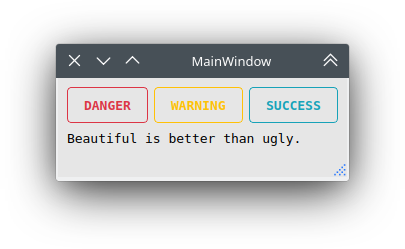
\includegraphics[width=0.6\textwidth]{Appendix/python_modules/Figures/qt-extra.png}
\par\end{centering}
\caption{QPushButtons stylized with class property.}
\label{fig:qt-extra}
\end{figure}

%======================================================================
\section{Custom stylesheets}
Custom changes can be performed by overwriting the stylesheets, for example:
\begin{python}
QPushButton {{
  color: {QTMATERIAL_SECONDARYCOLOR};
  text-transform: none;
  background-color: {QTMATERIAL_PRIMARYCOLOR};
}}

.big_button {{
  height: 64px;
}}
\end{python}
Then, the current stylesheet can be extended just with:
\begin{python}
apply_stylesheet(app, theme='light_blue.xml')

stylesheet = app.styleSheet()
with open('custom.css') as file:
    app.setStyleSheet(stylesheet + file.read().format(**os.environ))
\end{python}
And the class style can be applied with the \quot{setProperty} method:
\begin{python}
self.main.pushButton.setProperty('class', 'big_button')
\end{python}

\begin{figure}[H]
\begin{centering}
% \includesvg[width=0.8\textwidth]{Cap4/Figures/transformer.svg}
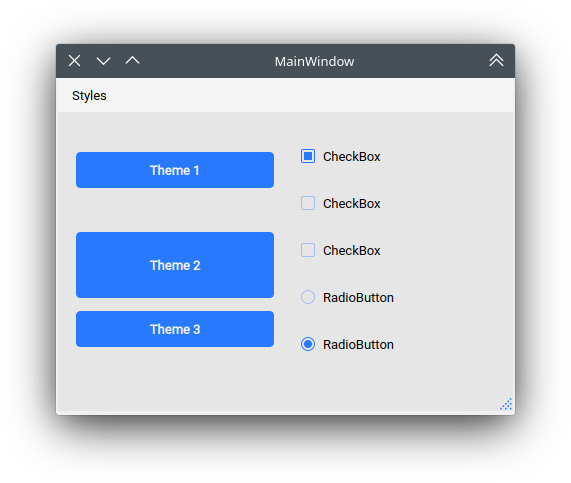
\includegraphics[width=0.7\textwidth]{Appendix/python_modules/Figures/qt-custom.png}
\par\end{centering}
\caption{QPushButtons stylized with user defined class property.}
\label{fig:qt-custom}
\end{figure}

%======================================================================
\section{Run examples}\
A window with almost all widgets (see the previous screenshots) are available to test all themes and create new ones.
\begin{python}
git clone https://github.com/UN-GCPDS/qt-material.git
cd qt-material
python setup.py install
cd examples/full_features
python main.py --pyside6
\end{python}

%======================================================================
\section{Change theme in runtime}
There is a \quot{qt\_material.QtStyleTools} class that must be inherited along to QMainWindow for change themes in runtime using the \quot{apply\_stylesheet()} method.
\begin{python}
class RuntimeStylesheets(QMainWindow, QtStyleTools):
    
    def __init__(self):
        super().__init__()
        self.main = QUiLoader().load('main_window.ui', self)
        
        self.apply_stylesheet(self.main, 'dark_teal.xml')
        # self.apply_stylesheet(self.main, 'light_red.xml')
        # self.apply_stylesheet(self.main, 'light_blue.xml')
\end{python}

%======================================================================
\section{Integrate stylesheets in a menu}
A custom stylesheets menu can be added to a project for switching across all default available themes.
\begin{python}
class RuntimeStylesheets(QMainWindow, QtStyleTools):
    
    def __init__(self):
        super().__init__()
        self.main = QUiLoader().load('main_window.ui', self)
        
        self.add_menu_theme(self.main, self.main.menuStyles)
\end{python}


%======================================================================
\section{Create new themes}
A simple interface is available to modify a theme in runtime, this feature can be used to create a new theme, the theme file is created in the main directory as \quot{my\theme.xml}
\begin{python}
class RuntimeStylesheets(QMainWindow, QtStyleTools):
    
    def __init__(self):
        super().__init__()
        self.main = QUiLoader().load('main_window.ui', self)
        
        self.show_dock_theme(self.main)
\end{python}
A full set of examples are available in the \citefoot{exmaples directory}{https://github.com/UN-GCPDS/qt-material/blob/master/examples/runtime/}

%======================================================================
\section{Export theme}
This feature able to use \textit{Qt-Material} themes into \quot{Qt} implementations using only local files.
\begin{python}
from qt_material import export_theme

extra = {

    # Button colors
    'danger': '#dc3545',
    'warning': '#ffc107',
    'success': '#17a2b8',

    # Font
    'font_family': 'monoespace',
    'font_size': '13px',
    'line_height': '13px',

    # Density Scale
    'density_scale': '0',

    # environ
    'pyside6': True,
    'linux': True,

}

export_theme(theme='dark_teal.xml', 
             qss='dark_teal.qss', 
             rcc='resources.rcc',
             output='theme', 
             prefix='icon:/', 
             invert_secondary=False, 
             extra=extra,
            )
\end{python}
This script will generate both \quot{dark\_teal.qss} and \quot{resources.rcc} and a folder with all theme icons called \quot{theme}.

The files generated can be integrated into a \quot{PySide6} application just with:
\begin{python}
import sys

from PySide6 import QtWidgets
from PySide6.QtCore import QDir
from __feature__ import snake_case, true_property

# Create application
app = QtWidgets.QApplication(sys.argv)

# Load styles
with open('dark_teal.qss', 'r') as file:
    app.style_sheet = file.read()

# Load icons
QDir.add_search_path('icon', 'theme')

# App
window = QtWidgets.QMainWindow()
checkbox = QtWidgets.QCheckBox(window)
checkbox.text = 'CheckBox'
window.show()
app.exec()
\end{python}
This files can also be used into non \quot{Python} environs like \quot{C++}.

%======================================================================
\section{Density scale}
The \quot{extra arguments} also include an option to set the \textit{density scale}, by default is \quot{0}.
\begin{python}
extra = {
    
    # Density Scale
    'density_scale': '-2',
}

apply_stylesheet(app, 'default', invert_secondary=False, extra=extra)
\end{python}
